%
% hyperbola.tex -- hyperbolas
%
% (c) 2019 Prof Dr Andreas Müller, Hochschule Rapperswil
%
\documentclass[tikz,12pt]{standalone}
\usepackage{amsmath}
\usepackage{times}
\usepackage{txfonts}
\usepackage{pgfplots}
\usepackage{csvsimple}
\usetikzlibrary{arrows,intersections,math}
\begin{document}
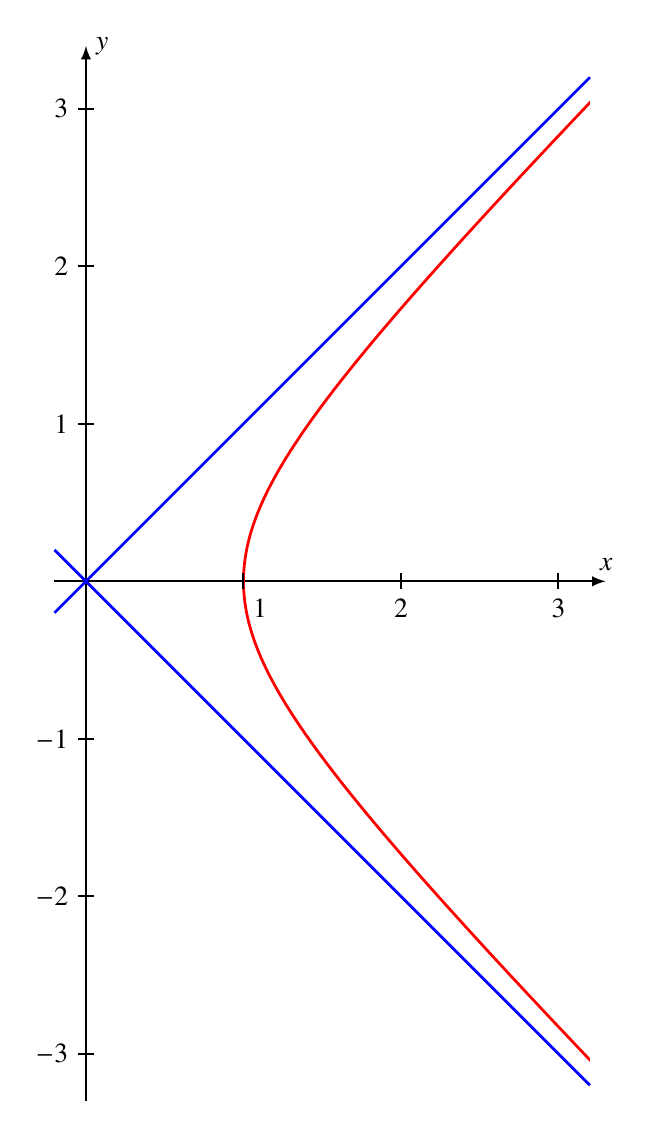
\begin{tikzpicture}[>=latex,scale=2]

\draw[->,line width=0.7pt] (-0.2,0)--(3.3,0) coordinate[label={$x$}];
\draw[->,line width=0.7pt] (0,-3.3)--(0,3.4) coordinate[label={right:$y$}];

\draw[color=blue,line width=1pt] (-0.2,-0.2)--(3.2,3.2);
\draw[color=blue,line width=1pt] (-0.2, 0.2)--(3.2,-3.2);

\begin{scope}
\clip (0,-3.2) rectangle (3.2,3.2);
\draw[color=red,line width=1pt]
	plot[domain=-2:2,samples=100]
		({0.5*(exp(\x)+exp(-\x))},{0.5*(exp(\x)-exp(-\x))});
\end{scope}

\foreach \t in {1,...,3}{
	\draw[line width=0.7pt] ({\t},-0.05)--({\t},0.05);
	\draw[line width=0.7pt] (-0.05,{\t})--(0.05,{\t});
	\draw[line width=0.7pt] (-0.05,{-\t})--(0.05,{-\t});
	\node at (-0.05,{\t}) [left] {$\t$};
	\node at (-0.05,{-\t}) [left] {$-\t$};
}
\node at (1,-0.05) [below right] {$1$};
\node at (2,-0.05) [below] {$2$};
\node at (3,-0.05) [below] {$3$};

\end{tikzpicture}
\end{document}

